% \chapter{Verification Plan for a Full Development}
% \label{sec:verification-plan-full}

\nthng{
\texttt{Contributors to this chapter:
  \begin{description}
  \item[DLR] Overall coherence, revise structure of the Verification Report
  \item[All4Tec] Role of model-based testing, \qq{hopefully more}
  \item[SQS] Overall coherence
  \item[CEA] Tools and methods Sec.~\ref{sec:methods-tools})
  \item[U Bremen] Tools and methods (model based testing, bounded
    model checking Sec.~\ref{sec:methods-tools}),
    V\&V process steps
  \item[Fraunhofer] Tools and methods Sec.~\ref{sec:methods-tools})
  \item[TUBS] Safety Interface, general tool list
  \item[TWT, URO] Tools and methods Sec.~\ref{sec:methods-tools})
  \item[DB, SNCF, NS] operator role (end user scenarios, validation
    requirements and contribution)
  \item[Institut Telecom] Methods and Tools Sec.~\ref{sec:methods-tools})
  \end{description}
}
}

The section is going to instantiate the generic \VV plan from the standard to
the EVC development in openETCS-style (FLOSS). This entails the organisation,
a definition of the requirements, 
generic schedule covering all design steps, resources, responsibilities, 
tools, techniques, and methodologies to be 
deployed in order to perform the verification activities, and all the
documents which are to be produced.

The result must conform to the requirements of the standards for a
SIL~4 development.

  As D2.3 gives only a rough description of the development steps and
  not yet a complete list of design artifacts, nor one of methods
  applied and formats to be used, this first version (V01) of the V\&V plan
  will also lack detail which will to be added in later revisions as
  these informations become more concrete.

\section{\VV Plan Overview}
\label{sec:plan-overview}

This section gives an overview of the \vv plan for a full development. 

\subsection{\VV Organisation}
\label{sec:vv-organisation}

This section defines the relationship of verification and validation
to other efforts such as development, project management, quality
assurance, and configuration management. It defines the lines of
communication within the \vv, the authority for resolving issues, and
the authority for approving \vv deliverables. Here, the \vv aspect of
the ``openETCS-ecosystem'' should be outlined.



\subsection{\VV Activity Overview}
\label{sec:vv-activity-overview}

This section gives a short overview of the activities (Verification or
Validation) which happen at the respective development steps, to be
detailed in the subsequent sections. The numbering (e.g.\ 2e) refers
to Fig.~\ref{fig:openETCSProcess}. Abbreviations used are defined in
the glossary, Sec.~\ref{sec:glossary}.

\begin{description}
\item[SSRS---Verification (1c):] verification that the SSRS the requirements
  consistently extends the requirements base. 
\item[SSRS---Validation (1c):] Deriving a sub-system test specification
\item[SFM---Verification (2c):] Verification that the model formalises
  the requirements
\item[SFM---Validation (2c):] Detailing the test specification,
  perhaps validating the model (e.g.\ via animation)
\item[SW-SFM---Verification (3d):] Verifying the SW-HW architecture
  definition (should be somewhere) and the software model
\item[SW-SFM---Validation (3d):]Perhaps validation of the software model
\item[SW-FFM---Verification (3d):]  verification, employing also
  formal methods/tools 
\item[SW-FFM---Validation (3d):] validation, may e.g.\ employ model checkers
\item[Code---Verification (3e):] verification depends on the code
  generation method (manual, generated, generated with validated
  tool), unit test requirements have to be met, afterwards code
  integration tests
\item[Code---Validation (3e):] no specific activities foreseen
\end{description}

The following step descriptions are preliminary and shall serve as a
concept which is to be detailed in later revisions (V02 and up).
%
\begin{description}
\item[EVC Software---Verification (tbd):] Perform software system verification
\item[EVC Software---Validation (tbd):] Validation against user
  requirements/scenarios, broken down to software functionality
\item[SW/HW integration (tbd):] Use the API in a simulation
  environment as a replacement of actual SW/HW integration
\item[Final Validation (tbd):] Apply user (railway operator) requirements and scenarios (based
  on the sub-system test specification)
\end{description}

\subsection{Schedule}
The overview of the activities given above shalle be detailed in this
section. The objective here is to define an orderly flow of material
between project activities and verification tasks.  

\nthng{It describes the project life cycle and project milestones
  including completion dates.  Summarize the schedule of verification
  tasks and how verification results provide feedback to the whole
  openETCS process to support overall project management functions.
  The objective of this section is to define an orderly flow of
  material between project activities and verification tasks.}

\subsection{\VV Resources}
\label{sec:vv-resources}

In a regular development project, resources needed to perform
verification tasks, including staffing, facilities, tools, finances,
and special procedural requirements such as security, access rights,
and documentation control, have to be defined. Here, where we define
merely a pattern of a V\&V plan, the emphasis will lie on spelling out
requirements and proposing
principal solutions.
\nthng{  
\textit{Guidance: This section summarizes the resources needed to
  perform verification tasks, including staffing, facilities, tools,
  finances, and special procedural requirements such as security,
  access rights, and documentation control.}
}

\subsection{Responsibilities}
\label{sec:vv-responsibilities}

\nthng{
\textit{Guidance: Identify the organization responsible for performing Verification tasks. There are two levels of responsibility--- 
general responsibilities and specific responsibilities for the verification tasks to be performed should be assigned to individuals. Here, in the general \vv plan, only the first are to be defined.}
}
\begin{center}
\begin{longtable}{|m{2,5cm}|m{6cm}|m{2cm}|m{2cm}|}
\caption{General \VV Responsibilities}
\label{tab:gener-vv-respo}\\

\hline \rowcolor{myblue} \multicolumn{1}{|c|}{Role} &
\multicolumn{1}{|c|}{Name of the person} &
\multicolumn{1}{|c|}{Affiliation} & \multicolumn{1}{|c|}{Activity
  Code} \\ \hline
\endfirsthead

\multicolumn{4}{c}%
{{\bfseries \tablename\ \thetable{} -- continued from previous page}} \\
\rowcolor{myblue} \multicolumn{1}{|c|}{Role} &
\multicolumn{1}{|c|}{Name of the person} &
\multicolumn{1}{|c|}{Company} & \multicolumn{1}{|c|}{Activity Code} \\
\hline
\endhead

\hline \multicolumn{4}{|r|}{{Continued on next page}} \\ \hline
\endfoot

\hline \hline
\endlastfoot

Verification Team Manager & & & \\\hline
Verifier & & & \\\hline
\end{longtable}
\end{center}

\section{Requirements Base}
\label{sec:requirements-base}

This section shall provide references to all requirements 
against which the design is to be verified and validated. It does not include 
process requirements. For the latter, see Sec.~\ref{sec:appendix}.

The requirements on the EVC software origin in the SS-026 and TSI
specifications.




\section{Verification Acitivities for a Full Development}
\label{sec:verif-full-devel}

\textit{for each of the verification steps identified in the plan
  overview, the following has to be instantiated: }
\subsection{DAS2V Verification}
\label{sec:dasv-verification}

\subsubsection{Task}
\label{sec:dasv-verif-task}

\subsubsection{Documents to Be Produced}
\label{sec:dasv-verif-docum-be-prod}

\subsubsection{Phase Specific Activities}
\label{sec:dasv-verif-phase-spec-activ}

\subsubsection{Techniques and Measures}
\label{sec:dasv-verif-techniques-measures}

\textit{Here the verification plan begins}

\subsection{SSRS Verification (1c)}
\label{sec:ssrs-verification}

\subsubsection{Task}
\label{sec:ssrs-verif-task}

The SSRS (sub-system requiement specification) outlines the subsystem
which is going to be modeled within the project. The SSRS describes
the architecture of the subsystem (functions and their I/O) and the
requirements allocated to these functions. If necessary, the
requirements are rewritten in order to address the I/O and to
correspond to the allocation. It also provides the classification into
vital and non vital requirements and data
streams. The architecture part is described in a semi-formal language,
and the requirements are described in natural language.

The SSRS is to be viewed as a supplement to the SS-026 and the
TSIs and is not intended to replace them. The verification has to
check that a complete and consistent set of functionalities have been
identified and that the architecture is adequate. 

%\todo{Verifiy hazard analysis too?}


\subsubsection{Documents to Be Produced}
\label{sec:ssrs-verif-docum-be-prod}

SSRS verification report.

\subsubsection{Phase Specific Activities}
\label{sec:ssrs-verif-phase-spec-activ}

\subsubsection{Techniques and Measures}
\label{sec:ssrs-verif-techniques-measures}

 Due to the informal
nature of the SSRS, mainly manual techniques are to be applied.

\qq{Review}



\subsection{SFM Verification (2c)}
\label{sec:sfm-verif-verification}

\subsubsection{Task}
\label{sec:sfm-verif-task}

\subsubsection{Documents to Be Produced}
\label{sec:sfm-verif-docum-be-prod}

\subsubsection{Phase Specific Activities}
\label{sec:sfm-verif-phase-spec-activ}

\subsubsection{Techniques and Measures}
\label{sec:sfm-verif-techniques-measures}




%\todo{further verification phases}

\subsection{System Verification}
%\textcolor{red}{<Brief Introduction>}

\paragraph{SSRS Verification(1c)}
The SSRS Verification phase refers to the task already defined in the
Sec.~\ref{sec:ssrs-verification} of this document that involves the
full development.  For further details about the activities involved,
please go to the mentioned section.

\subsubsection{Software Verification}
\label{sec:sw-verif}

This section describes software verification activities in greater
detail than the description above. This presentation of the material
shall be unified in due course.

The SW process is detailed in the D.2.3 OpenETCS process. Bearing in
mind that the tasks described in this openETCS Verification plan are
strongly linked to the Software process defined in that document, the
following figure is included in order to have present the key points
to be covered in the plan.

\begin{figure}[h]
  \centering
  \fbox{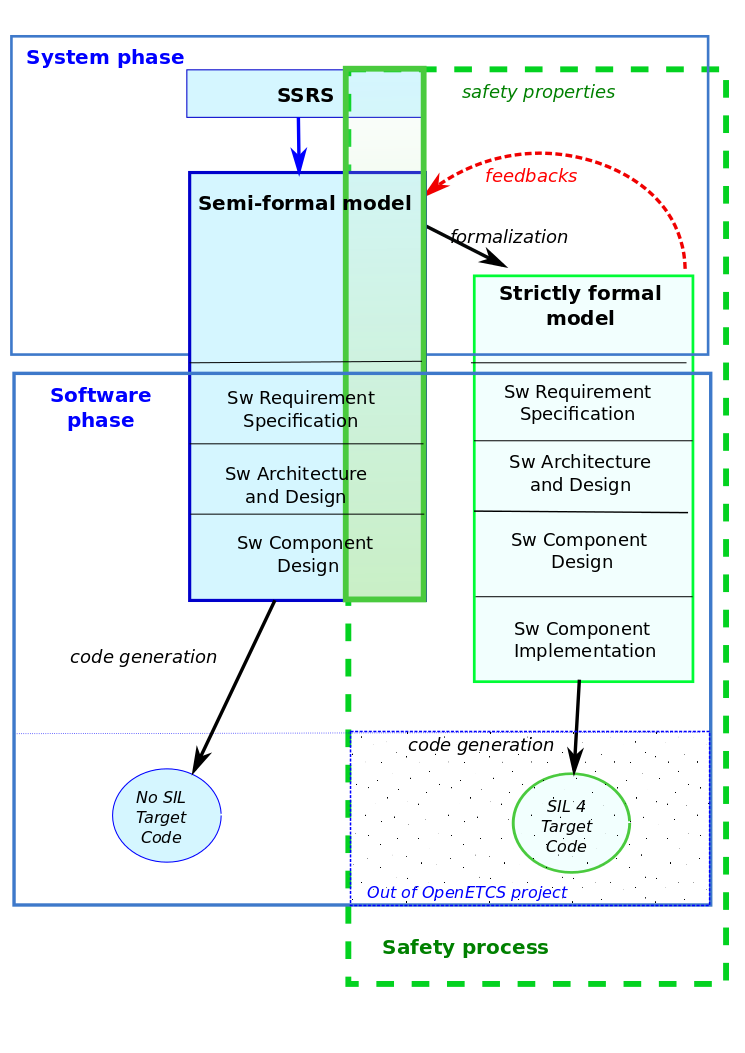
\includegraphics[width=4in]{Model-phase.png}}
  \caption{Software phase description}
  \label{fig:detailed software}
\end{figure}

\textbf{SW Requirements Verification}

\underline{Task} 

In the SW Requirements Specification the SSRS shall be taken as
starting point, redefining it to ensure the software constraints are
considered.  The SW Requirements Verification phase then shall verify
that the proposed Software Requirements cover as much as possible of
the SSRS and provide a correct implementation of the System
Requirements in the Software context.  On the other hand, the
Verification done in this phase shall include the assessment of the SW
Requirements modelling, the objective is to ensure the representation
of the requirements is coherent with their specification as well as
complete, explicit and implementable, as well as traceable to the
semi-formal and/or formal models defined in the system phase.

\underline{Documents to Be Produced} 

\begin{itemize}
\item SW Requirements Verification Report
\end{itemize}

\underline{Activities}

Some activities shall be performed to ensure the requirements are
written in a readable and testable manner. The Verification of the
Software Requirements shall assess whether the requirements met the
following aspects:
\begin{itemize}
\item Deterministic: Given an initial system state and a set of
  inputs, you must be able to predict exactly what the outputs will
  be.
\item Unambiguous: All openETCS project members must get the same
  meaning from the requirements; otherwise they are ambiguous.
\item Correct: The relationships between causes and effects are
  described correctly.
\item Complete: All requirements are included. There are no omissions.
\item Non-redundant: Just as the Software modelling (semi-formal and
  formal) provides a non-redundant set of data, the requirements
  should provide a non-redundant set of functions and events.
\item Lends itself to change control: Requirements, like all other
  deliverables of the openETCS project, should be placed under change
  control.
\item Traceable: SW Requirements must be traceable to each other, to
  the SSRS, to the objectives, to the design, to the test cases, and
  to the code.
\item Readable by all project team members: The project stakeholders,
  including the users, experts and testers, must each arrive at the
  same understanding of the requirements.
\item Written in a consistent style: Requirements should be written in
  a consistent style to make them easier to understand.
\item Explicit: Requirements must never be implied.
\item Logically consistent: There should be no logic errors in the
  relationships between causes and effects.
\item Lends itself to reusability: Good requirements can be reused on
  future projects based on openETCS.
\item Succinct: Requirements should be written in a brief manner, with
  as few words as possible.
\item Annotated for criticality: Each SW requirement should note the
  level of criticality to the openETCS project. In this way, the
  priority of each requirement can be determined, and the proper
  amount of emphasis placed on developing and testing each
  requirement.
\item Feasible: If the software design is not capable of delivering
  the requirements, then the requirements are not feasible.
\end{itemize}

The activities that shall ensure these aspects are successfully met
are the following:
\begin{itemize}
\item {\it SWReq-Ver-Act1. Compliance with SSRS}: the SW Requirements
  are based on the SSRS, so it shall be ensured that their
  specification is compliant and coherent with regard to the SSRS; the
  SW requirements complement, adjust and enlarge the scope delimited
  by the SSRS in the Software phase.
\item {\it SWReq-Ver-Act2. Accuracy, Consistency, Completeness,
    Correctness assurance}: A significant problem with recording
  requirements as text is the difficulty of analyzing them for
  completeness, consistency, and correctness. The Specification of the
  SW Requirements has precise syntactic and semantic rules (e.g., data
  type consistency) and the specification of the requirements shall be
  compared against those established rules to ensure these aspects are
  correctly covered.
\item {\it SWReq-Ver-Act3. Testability assurance}: The two objectives
  for testing the openETCS safety-critical SW are the demonstration
  that the software satisfies its requirements and the demonstration
  that errors that could lead to unacceptable failures have been
  removed.
\item {\it SWReq-Ver-Act4. Verificability assurance}: The SW
  Requirements shall identify the main functionality and describe the
  functional breakdown and data flows from top-level functions to
  low-level functions. The description provided as well as the flows
  identified shall be verifiable.
\item {\it SWReq-Ver-Act5. Compliance with Standards}: Compliance with
  CENELEC Standards (EN50126, EN50128 and EN50129) shall be verified.
\item {\it SWReq-Ver-Act6. Traceability with SSRS}: Each SSRS
  allocated to software must map to one or more software
  requirement. Traceability analysis, which can be automated,
  determines the completeness of the mapping of SSRS to software. A
  table similar to this one shall be obtained, either manually or
  automatically to assess the conformance with this expected activity.
\item {\it SWReq-Ver-Act7. Requirements modelling correctness}:
  Considering "the result of the modelling activities is a document
  that represents a thorough understanding of the problem the proposed
  software is intended to solve"\textcolor{red}{[1. Cho, Chin-Kuei,
    Quality Programming, John Wiley \& Sons, Inc, 1987, p 21.]},
  during the SW Requirements verification, it shall be possible to
  capture all required information, including additional information
  for safety-critical aspects with the support of the models. These
  Requirements representations shall be compared to their original
  specification and assess whether they are complete and enough to
  cover all the information provided by them.
\end{itemize}

\begin{center}
\begin{longtable}{|m{5cm}|m{7cm}|}
  \caption{Requirements Trace Table}\\
  \hline \rowcolor{myblue} \multicolumn{1}{|c|}{Source SSRS ID} &
  \multicolumn{1}{|c|}{SW Requirement ID} \\ \hline
\endfirsthead
\multicolumn{2}{c}%
{{\bfseries \tablename\ \thetable{} -- continued from previouqs page}} \\
\rowcolor{myblue} \multicolumn{1}{|c|}{Source SSRS ID} &
\multicolumn{1}{|c|}{SW Requirement ID} \\ \hline
\endhead
\hline \multicolumn{2}{|r|}{{Continued on next page}} \\ \hline
\endfoot
\hline \hline
\endlastfoot
SSRS-xxxx &
SWR-yyy
\\\hline
SSRS-xxxx &
SWR-yyy
\\\hline
\end{longtable}
\end{center}

\underline{Tools, Techniques, Methods and Measures} 

This section shall identify the special software tools, techniques, and
  methodologies to be employed by the verification team. 
The purpose of each should be defined and plans for the acquisition,
training, support, and qualification of each shall be described in
this section.

The following table summarizes the Techniques, methods, measures or
tools proposed for the identified activities. 

\begin{center}
\begin{longtable}{|m{1,5cm}|m{8,5cm}|m{4cm}|}
  \caption{SW Requirements Verification Tools, Techniques, Methods and Measures}\\
  \hline \rowcolor{myblue} \multicolumn{1}{|c|}{Activity} &
  \multicolumn{1}{|c|}{Techniques/ Methods/ Measures} &
  \multicolumn{1}{|c|}{Tools}\\ \hline
\endfirsthead
\multicolumn{3}{c}%
{{\bfseries \tablename\ \thetable{} -- continued from previous page}} \\
\rowcolor{myblue} \multicolumn{1}{|c|}{Activity} &
\multicolumn{1}{|c|}{Techniques/ Methods/ Measures} &
\multicolumn{1}{|c|}{Tools} \\\hline
\endhead
\hline \multicolumn{3}{|r|}{{Continued on next page}} \\ \hline
\endfoot
\hline \hline
\endlastfoot
{\it SWReq-Ver-Act1} & 
This compliance is verified by peer review. The first version of SW
Requirements is usually incomplete and composed primarily of top-level
adjustments. The meaning of the SW requirements is described
textually. & 
<To be defined>  
\\\hline
{\it SWReq-Ver-Act2} & 
Since the modelling at this stage is provided, verification is mostly
based on review and with a tools-based modelling approach. Some
consistency checks between the SW Requirements and both the
semi-formal modelling and the formal modelling can be automated. 
& 
<To be defined>  
\\\hline
{\it SWReq-Ver-Act3} &
Requirements-based testing has been found to be effective at revealing
errors early in the testing process Requirement models created with
standard UML use-case notations are not robust enough to create
requirements based test cases that met the safety-critical aspects, so
the standard use-case model notation shall be extended to allow the
capture of additional information required to determine test cases. & 
Test cases can be automatically generated from ``test-ready'' use-case
models. <To be defined>   
\\\hline
{\it SWReq-Ver-Act4} & 
Verification is mostly based on review &
<To be defined> 
\\\hline
{\it SWReq-Ver-Act5} & 
Verification is mostly based on review &
<To be defined>
\\\hline
{\it SWReq-Ver-Act6} & 
A traceability matrix between SSRS and SW Requirements shall be
prepared either manually or automatically and assessed by review &  
Integrated tools can generate software to system requirements
traceability tables showing which software requirements are allocated
to system requirements. <To be defined> 
\\\hline
{\it SWReq-Ver-Act7} & 
Verification is mostly based on review & 
<To be defined>
\\\hline
\end{longtable}
\end{center}

\textbf{SW Architecture, Design and Modelling Verification}

\underline{Task} 

This phase aims to ensure that the software architecture design
adequately fulfils the software requirements specification already
verified in the SW Requirements Verification phase. 
The software architecture defines the major elements and subsystems of
the openETCS software, how they are interconnected, and how the
required (safety integrity) attributes will be achieved. It also
defines the overall behaviour of the software, and how the software
elements interact.  
To carry this phase the information from the current software
lifecycle phase shall be verified. All essential information should be
available and must be verified; the information should include the
adequacy of the specifications, design and plans in the current phase.  
The architecture and design shall be modelled and the coherence of
those models with regard to their specification shall be verified to
assess whether the constraints are correctly treated. 
The verification configuration should be precisely defined and the
verification activities shall be repeatable. 

\underline{Documents to Be Produced} 

\begin{itemize}
\item SW Architecture, Design and Modelling Verification Report
\end{itemize}

\underline{Activities}

Software architecture verification should consider whether the
software architecture design adequately fulfils the SW requirements
specification.  

The essential properties to be verified during this phase are:

\begin{itemize}
\item What is the software supposed to do: including the SW
  specification and the system capabilities
\item What is the software not supposed to do: be aware of the
  unexpected emergent behaviour, boundary specifications, inhibits
\item What is the software supposed to do under adverse conditions:
  system biases, tolerances
\item What are the safety considerations
\item What are the integration or interfacing considerations:
  subsystems, modules, components, relationship between hardware and
  software, partitions, parallelism, compatibility 
\item What are the dependability considerations: performance,
  capacity, complexity, stability
\end{itemize}

Considering these aspects, a table shall be prepared to list a
relation of verification dimensions regarding to the Architecture and
Design that facilitates the process. An example is given below:

\begin{center}
\begin{longtable}{|m{2cm}|m{2cm}|m{2,1cm}|m{2cm}|m{1cm}|m{2cm}|m{2,1cm}|}
\caption{SW Architecture Verification preparation table - Example of contents}\\
\hline \rowcolor{myblue} \centering \textbf{Verification dimension} &
\centering \textbf{Intended behaviour} & \centering
\textbf{Unacceptable behaviour} & \centering \textbf{Adverse
  conditions} & \centering \textbf{Safety} & \centering
\textbf{Integration} & \textbf{Dependability} \\\hline  
\endfirsthead
\multicolumn{7}{c}%
{{\bfseries \tablename\ \thetable{} -- continued from previous page}} \\
\rowcolor{myblue} \centering \textbf{Verification dimension} &
\centering \textbf{Intended behaviour} & \centering
\textbf{Unacceptable behaviour} & \centering \textbf{Adverse
  conditions} & \centering \textbf{Safety} & \centering
\textbf{Integration} & \textbf{Dependability} \\\hline  
\endhead
\hline \multicolumn{7}{|r|}{{Continued on next page}} \\ \hline
\endfoot
\hline \hline
\endlastfoot
Performance analysis & Service delivery & Consequences of service
failure, unexpected emergent behaviour & Distributed redundancy and
fail-over & & &   
\\\hline
Timing Requirements & normal behaviour & Blown performance margins,
missing timing requirements & Distributed redundancy and fail-over &
Safety and Recoverability, timing margins & Timeline  
management, phase transition interlocks &   
\\\hline
Security Requirements & Secure communication & Compromised
communication & Redundant communication channels & & &  
\end{longtable}
\end{center}
The software architecture modelling, which consists of determining and
connecting software components, requires a phase of analysis to be
able to validate the representation carried out, as errors can occur
in the representation. It is thus necessary to be able to identify and
to provide them to the designer.  

Modelling must also bring answers in term of feasibility and the
constraint shall be analyzed so the interdependent functions should
not overlap.

The verifications done at the software architecture level are related
to specification and execution model coherency.

The expected activities for this phase are the following:
\begin{itemize}
\item {\it SWArch-Ver-Act1. Check the software architecture design}:
  The SW architecture and design should fulfil the SW requirements
  specification. From a safety point of view, the software
  architecture phase is where the basic safety strategy for the
  software is developed. 
\item {\it SWArch-Ver-Act2. Handle attributes}: The attributes of
  major elements and subsystems should be adequate with reference to
  the feasibility of the safety performance required, testability for
  further verification, readability by the development and
  verification team, and safe modification to permit further
  evolution. With the attributes, on which we rely once the software
  is specified, it is possible to check if the model of execution and
  the coherence of the periods of the various software components are
  corrects. 
\item {\it SWArch-Ver-Act3. Check incompatibilities}: The
  incompatibilities between design and specification should be
  checked.  
\item {\it SWArch-Ver-Act4. Model coherency}: Verify the
  representation carried out with the modelling. The errors identified
  can be related to the symmetry of the inter-connected functions. A
  certain number of constraints of coherence must thus be analyzed.  
\item {\it SWArch-Ver-Act5. Constraints analysis}: Ensure system
  dysfunctions do not occur. Some components can also execute an
  operation depending on a signal resulting from another component,
  which results in constraints of synchronization that must also be
  taken into account.  

\end{itemize}

\underline{Tools, Techniques, Methods and Measures} 

The specific software tools, techniques, and methodologies to be
employed by the verification team are to be identified here.  The
purpose of each should be defined and plans for the acquisition,
training, support, and qualification of each shall be described in
this section.

The following table summarizes the Techniques, methods, measures or
tools proposed for the identified activities.

\begin{center}
\begin{longtable}{|m{1,5cm}|m{8,5cm}|m{4cm}|}
\caption{SW Architecture, Design and Modelling Verification Tools,
  Techniques, Methods and Measures}\\ 
\hline \rowcolor{myblue} \multicolumn{1}{|c|}{Activity} &
\multicolumn{1}{|c|}{Techniques/ Methods/ Measures} &
\multicolumn{1}{|c|}{Tools}
\\ \hline 
\endfirsthead
\multicolumn{3}{c}%
{{\bfseries \tablename\ \thetable{} -- continued from previous page}} \\
\rowcolor{myblue} \multicolumn{1}{|c|}{Activity} &
\multicolumn{1}{|c|}{Techniques/ Methods/ Measures} &
\multicolumn{1}{|c|}{Tools} 
\\\hline
\endhead
\hline \multicolumn{3}{|r|}{{Continued on next page}} \\ \hline
\endfoot
\hline \hline
\endlastfoot
{\it SWArch-Ver-Act1} & 
 & 
<To be defined> 
\\\hline
{\it SWArch-Ver-Act2} & 
&  
<To be defined> 
\\\hline
{\it SWArch-Ver-Act3} &
&
<To be defined> 
\\\hline
{\it SWArch-Ver-Act4} & 
 &
<To be defined> 
\\\hline
{\it SWArch-Ver-Act5} & 
 &
<To be defined> 
\\\hline
\end{longtable}
\end{center}

\textbf{SW Component and Modelling Verification}

\underline{Task} 

This phase analyzes whether the SW components defined in the openETCS
Software process are verifiable by design, with a focus on the formal
verification of data aspects of components and components modelling.
This task requires a detailed understanding not only of the
corresponding specification, but also the environments and methodology
in which the verification component will be used.

This phase delivers methods and tools to

\begin{itemize}
\item Verify the component models by model-checking techniques, with a
  focus on behavioural aspects such as attributes and data-dependent
  properties 
\item Verify the specification of the components is coherent to the SW
  architecture and design previously verified. This activity shall be
  based on the existing models in the component stage as well as
  previous phases, in close connection with the model checking
  activities. 
\end{itemize}

\underline{Documents to Be Produced} 

\begin{itemize}
\item SW Component and Modelling Verification Report
\end{itemize}

\underline{Activities}

This phase aims to assess whether the specification and modelling of
components are reusable, configurable, and implementable in the
expected code automatically generated environment.

\begin{itemize}
\item Within the context of the models that contain the components
  identified for the SW phase, the verification of components within a
  control system model shall be required.  As standalone components ---
  For a high level of confidence in the component algorithm, verify
  the component in isolation from the rest of the components and
  sub-systems identified. This approach is called component analysis.
\item Verifying standalone components provides several advantages:
\begin{itemize}
\item The analysis can be be used to focus on portions of the design
  that cannot be tested because of the physical limitations of the
  system being controlled.
\item This approach can be used for open-loop simulations to test the
  plant model without feedback control.
\end{itemize}
\end{itemize}

The components shall be identified at the points of minimal coupling
(minimal control and/or information exchange) and decompose the
specification. The smaller components might be amenable to be verified
and how to abstract these parts of the specification shall be
analysed.

The rest of the specification could be exposed to formal analysis,
such as model checking or theorem proving. The abstraction reduces the
number of states that need to be checked by an automated verification
technique and helps in avoiding the state explosion problem, which
occurs in traditional model checking.

An approach to specification decomposition is slicing the system
specifications represented with Petri Nets. In this way, the
specification shall improve the understanding of the complexity of the
system and high-risk components can be identified earlier.

The activities that shall ensure these aspects are successfully met
are the following:
\begin{itemize}
\item {\it SWComp-Ver-Act1. Verify components with minimal coupling
    independently of the model}: Within this activity a component
  analysis shall be performed to verify model blocks, atomic
  subsystems and statechart atomic subcharts. After extracting the
  blocks, or contents of the subsystems and subcharts, a harness model
  shall be created for the referenced model and the extracted model
  with the contents of the subsystem o subchart. A Test suite shall be
  prepared and executed to record coverage and output values. The Code
  Generation Verification (CGV) shall be invoked to execute the test
  cases on the generated code for the model that contains the
  component.
\item {\it SWComp-Ver-Act2. Verify components with minimal coupling in
    the context of the model}: A similar process shall be conducted in
  this case but performing a system analysis to verify the model
  blocks in the context of the model.
\item {\it SWComp-Ver-Act3. Formal analysis of components}: Perform
  model checking of components against properties; the results
  obtained shall highlight that: the component satisfies the
  properties for the environment; the component violates the
  properties for the environment; characterization of those
  environments in which the components satisfied each property.
\end{itemize}

Regarding the Modeling Verification, the activities involved shall ensure that:
\begin{itemize}
\item The models have been designed correctly and covers all the parts
  involved in the openETCS project
\item The algorithms have been implemented properly
\item The models do not contain errors, oversights, or bugs
\item The specification is complete and that mistakes have not been
  made in implementing the model
\end{itemize}

Each of the models defined in the full development context shall be
developed for a specific purpose and its validity is determined with
respect to that purpose. It shall be considered that a model that may
be valid for one set of conditions, can be invalid in another; because
of that, the model's output variables of interest shall be clearly
identified and their required amount of accuracy be specified.

It is costly and time consuming to determine whether a model is valid
over the complete domain of the full development context. Instead,
tests and evaluations are conducted until sufficient confidence and
certainty is obtained that a model can be considered valid. In the
model verification activities, tests are performed, errors are
identified, and corrections are made to the underlying models while
the models are exercised for the identified cases. Furthermore, the
verification of the models can result in retesting requirements to
ensure code integrity.

If the verification process determines that a model does not have
sufficient accuracy for any one of the sets of identified conditions,
then the model is invalid. However, determining that a model has
sufficient accuracy for numerous conditions does not guarantee that a
model is valid everywhere in its applicable domain.

\begin{itemize}
\item {\it SWModel-Ver-Act1.} 
\item {\it SWModel-Ver-Act2. }  
\item {\it SWModel-Ver-Act3. }
\end{itemize}

\underline{Tools, Techniques, Methods and Measures} 

The specific software tools, techniques, and methodologies to be
employed by the verification team are to be identified here. 
The purpose of each should be defined and plans for the acquisition,
training, support, and qualification of each shall be described in
this section. 

The following table summarizes the Techniques, methods, measures or
tools proposed for the identified activities.

\begin{center}
\begin{longtable}{|m{1,5cm}|m{8,5cm}|m{4cm}|}
\caption{SW Component and Modelling Verification Tools, Techniques,
  Methods and Measures}
\\
\hline \rowcolor{myblue} \multicolumn{1}{|c|}{Activity} &
\multicolumn{1}{|c|}{Techniques/ Methods/ Measures} &
\multicolumn{1}{|c|}{Tools}\\ \hline  
\endfirsthead
\multicolumn{3}{c}%
{{\bfseries \tablename\ \thetable{} -- continued from previous page}} \\
\rowcolor{myblue} \multicolumn{1}{|c|}{Activity} &
\multicolumn{1}{|c|}{Techniques/ Methods/ Measures} &
\multicolumn{1}{|c|}{Tools} \\\hline 
\endhead
\hline \multicolumn{3}{|r|}{{Continued on next page}} \\ \hline
\endfoot
\hline \hline
\endlastfoot
{\it SWComp-Ver-Act1} & 
 & 
<To be defined>  
\\\hline
{\it SWComp-Ver-Act2} & 
& 
<To be defined>  
\\\hline
{\it SWComp-Ver-Act3} &
 &
 <To be defined>  
\\\hline
{\it SWModel-Ver-Act1} & 
 &
<To be defined> 
\\\hline
{\it SWModel-Ver-Act2} & 
 &
<To be defined>
\\\hline
{\it SWModel-Ver-Act3} & 
 & 
<To be defined>
\\\hline

\end{longtable}
\end{center}

\textbf{SW code generation Verification}

\underline{Task} 

This phase analyzes whether the generated code from the model is
correct, robust, complete, coherent and reliable, with a focus on the
formal verification and on the equivalence of the model and the
generated code.

This phase delivers methods and tools to

\begin{itemize}
\item Verify the equivalence between the model and the generated code
  by equivalence testing and dynamic testing techniques
\item Verify the correctness of the translation algorithm and its implementation
\item Verify the complexity, coding guidelines and syntax of the
  generated code by static analysis techniques
\item Verify the robustness of the generated code
\end{itemize}

\underline{Documents to Be Produced} 

\begin{itemize}
\item SW Code Generation Verification Report
\end{itemize}

\underline{Activities}

When in the other phase the confidence in the correctness of the model
has been verified, it is necessary to have high confidence in the
generated code.

To achieve verified code generation, it is not sufficient to only
verify the code generation algorithm due to the implementation of the
algorithm might introduce errors as well. It is necessary to
distinguish between the correctness of the translation algorithm
itself and the correctness of its implementation.

Within the context of the Code Generation Verification, the code
generation verification approach shall utilize translation testing to
demonstrate that the execution semantics of the model are preserved
during production code generation, compilation and linking

The validity of the translation process, i.e. whether or not the
semantics of the model have been preserved during code generation,
compilation and linking, shall be determined by comparing the system
reactions

The activities that shall ensure these aspects are successfully met
are the following:
\begin{itemize}
\item {\it SWCode-Ver-Act1. Semantic Properties Verification}: For
  safety reasons, it is necessary that the generated code is
  semantically equivalent to the original model specification to
  ensure correct software and system behavior.

  During this activity, the semantics of the original model is
  preserved during the code generation shall be demostrated. This will
  verify that the transformation algorithm is correct.

\begin{figure}[h]
  \centering
  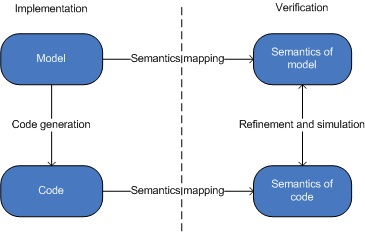
\includegraphics[scale=1]{images/transformation_verification.jpg}
  \caption{Transformation Verification}
  \label{fig:transformationver}
\end{figure}

To prove the semantical correctness of such a transformation, a
suitable model semantics is needed.

As a basic prerequisite, the semantics of the model and code must be
comparable and it is also required a semantics for both model and code
with the same semantic domain.

The first steps will be define the commom both model and code
semantics. A multitude of approaches can be taken to define such a
semantics. This definintion of the semantics poses subtle difficulties
due to inherent ambiguities. Once this is done the coverage over
semantics shall be identified.

Then, it will be necessary to establish a correspondence between the
model and code, based on refinement, and to prove it by simulation.

A refinement mapping correlating the control points of the model and
code, and indicating how the relevant model variables correspond to
the code variables or expressions at each control point shall be
established. For some transformation optimizations it is often
impossible to apply the refinement based rule since there are often no
control points where the states of the model and code can be
compared. So, a large class of these optimizations shall be identified
to allow their effective transformation verification.

After this, the simulation method shall be used for transformation verification. 

This transformation from model to code will be considered semantically
correct if the semantics of model and code are always the same.

Using the simulation principle to show that are equal, a simulation
relation in which they are contained shall be found and defined. Note
that the definition of a simulation relation is an artificial
construct for conducting proofs.


\item {\it SWCode-Ver-Act2.  Functional Correctness Verification}:
  Within this activity, as a first approach for functional properties
  correctness verification, the automatic test cases generated from
  the model will be executed under the automatic generated code from
  the same model, so that, the coherence, functionality and coverage
  of the code shall be verified.

  Taking into account the first obtained results, it will be possible
  to check the coverage of both code and test cases, detect the
  necessary functional properties not generated automatically, and
  they shall be inserted manually into the code.

  When discrepances are found, an analysis of both test cases and code
  shall be done to check in which part the problem is taking into
  account the techniques and tools of the specific verification phase
  activities.


\item {\it SWCode-Ver-Act3. Quality Properties (Complexity, Syntax,
    coding guidelines) Verification}: Within this activity, a static
  analysis shall be performed locating potentially vulnerable code.

  The static analysis involves no dynamic execution and will detect
  possible faults such as unreachable code, undeclared variables,
  parameter type mismatches, uncalled functions and procedures,
  possible array bound violations, standards fulfillment i.e. MISRA
  standard, etc.

The static analysis techniques will also include:
\begin{itemize}
\item \underline{data flow analysis}: it consists in a technique to
  follow the path that various specific items of data take through the
  code, looking for possible anomalies in the way the code handles the
  data items
\item \underline{control flow analysis}: technique for determining the
  control flow of the code. This type of analysis will identify
  infinite loops, unreachable code, cyclomatic complexity that
  identifies the number of decision points in a control flow, other
  complexity metrics like number of nested statements, etc.
\end{itemize}

With this analysis, errors in the structure and syntax of the code are
going to be found but run-time errors (errors that only occur when the
code is executed) will not be detected as we are not running the code.

Therefore this will not find things like memory leaks or check whether
a value in a variable is correct.

\item {\it SWCode-Ver-Act4. Equivalence Verification}: This activity
  shall use equivalence testing and other techniques like dynamic
  testing to demonstrate equivalence between the model and the
  generated code.
 
  During this phase, the execution of the model used for code
  generation and the object code derived from it with the same input
  stimuli followed by a comparison of the outputs shall be
  performed. The validity of the translation process, i.e. whether or
  not the semantics of the model have been preserved during code
  generation, compilation and linking, is determined by comparing the
  system reactions (results, which are the outputs resulting from
  stimulation with identical timed test inputs) of the model and the
  generated code.

  If the coverage achieved with the existing test inputs is not
  sufficient w.r.t. the selected model coverage metrics, additional
  test inputs that execute the model elements not covered shall be
  created. In practice, the tester can iteratively extend the set of
  test inputs using model coverage analysis until the chosen level of
  model coverage has been achieved. If full coverage for the selected
  metric(s) cannot be achieved, the uncovered parts shall be assessed
  and justification for uncovered parts shall be provided.
\item {\it SWCode-Ver-Act5. Robustness Verification}: Within this
  activity a code analysis shall be performed to verify its robustness
  so it behaves reasonably in exceptional situations; wrong execution
  paths, computational errors or erroneous inputs and memory
  alterations coming from the environment(errors caused by
  interactions between the software and its environment(hardware and
  software))

  The exceptional situations coming from the software itself can be
  automatically proven using static analyzers based on abstract
  interpretation such as Frama-C or RSM

  After this analysis, there will be necessary to check the
  exceptional situations coming from the environment. The
  inconsistencies between the specification and the user constrains
  present in the code shall be detected. To ensure the robustness of a
  piece of code, the value of each un-trusted input must be checked
  against its correctness domain after its production and before its
  consumption

  The robustness review of the generated code can be done by manual
  code review to verify that all checks are present at right locations
  and that the checked domains are strictly included in the
  correctness domains.
\end{itemize}

\underline{Tools, Techniques, Methods and Measures} 

The specific software tools, techniques, and methodologies to be
employed by the verification team are to be identified here. 
The purpose of each should be defined and plans for the acquisition,
training, support, and qualification of each shall be described in
this section. 

The following table summarizes the Techniques, methods, measures or
tools proposed for the identified activities.

\begin{center}
\begin{longtable}{|m{3cm}|m{7cm}|m{4cm}|}
\caption{SW Code Generation Verification Tools, Techniques, Methods
  and Measures}\\ 
\hline \rowcolor{myblue} \multicolumn{1}{|c|}{Activity} &
\multicolumn{1}{|c|}{Techniques/ Methods/ Measures} &
\multicolumn{1}{|c|}{Tools}\\ \hline  
\endfirsthead
\multicolumn{3}{c}%
{{\bfseries \tablename\ \thetable{} -- continued from previous page}} \\
\rowcolor{myblue} \multicolumn{1}{|c|}{Activity} &
\multicolumn{1}{|c|}{Techniques/ Methods/ Measures} &
\multicolumn{1}{|c|}{Tools} \\\hline 
\endhead
\hline \multicolumn{3}{|r|}{{Continued on next page}} \\ \hline
\endfoot
\hline \hline
\endlastfoot
{\it SWCode-Ver-Act1} & 
 & 
<To be defined>  
\\\hline
{\it SWCode-Ver-Act2} & 
& 
<To be defined>  
\\\hline
{\it SWCode-Ver-Act3} &
 &
 <To be defined>  
\\\hline
{\it SWCode-Ver-Act4} & 
 &
<To be defined> 
\\\hline
{\it SWCode-Ver-Act5} & 
 &
<To be defined>
\\\hline

\end{longtable}
\end{center}

\textbf{Traceability matrix Verification}

\underline{Task} 

The Traceability Matrix is a resource to ensure that the project's
scope, requirements, modeling and generated code remain as are
expected to be when compared to the objectives to be reached. The
matrix traces the different elements by establishing a thread for each
requirement to the corresponding model and component, the generated
code that consists on its implementations and the test cases defined.

\begin{itemize}
\item The specifications shall be verified following the traces
  between the elements defined in the matrix
\item With the matrix verification it shall be ensured that all the
  required information is included in the specification, such as
  process models and data models
\item Requirements that are not addressed by configuration items
  during design and code reviews can be identified; in a similar way,
  extra configuration items that are not required can be highlighted
\item The verification of the matrix shall provide input to change
  requests and future project plans when missing elements are
  identified
\end{itemize}

\underline{Documents to Be Produced} 

\begin{itemize}
\item Traceability Matrix Verification Report
\end{itemize}

\underline{Activities}

Taking the time to cross-reference each element involved in the
project to another element ensures that the results obtained by each
phase of the project are consistent with the requirements, the
modeling and the code.

To accomplish this objective it shall be verified that the
traceability matrix is in the following format:

\begin{itemize}

\item The matrix generated is a two-dimensional table,
\item There is one column per identified element (such as requirement,
model, components, or code),
\item A check mark at the end of the table shall be put if all the row
is well traced, coherent and unambiguous
\item Various traceability matrices may be utilized throughout the
project life cycle.  \item At least the matrices shall contain the
following elements:
\begin{itemize}
\item Formal specification of Requirements: It shows that each
requirement (obtained from SSRS) has been covered in an appropriate
section of the formal specification.
\item Design specification through modeling to functional
specification, this verifies that each function has been covered in
the design.
\item System test plan to functional specification ensures the test
case or test scenario for each process, component and each requirement
in the functional specification have been identified
\end{itemize}
\end{itemize}

\underline{Tools, Techniques, Methods and Measures}

The specific software tools, techniques, and methodologies to be
employed by the verification team are to be identified here.  The
purpose of each should be defined and plans for the acquisition,
training, support, and qualification of each shall be described in
this section.

The following table summarizes the Techniques, methods, measures or
tools proposed for the identified activities.

\begin{center}
\begin{longtable}{|m{1,5cm}|m{8,5cm}|m{4cm}|}
\caption{Traceability Matrix Verification Tools, Techniques, Methods
  and Measures}\\ 
\hline \rowcolor{myblue} \multicolumn{1}{|c|}{Activity} &
\multicolumn{1}{|c|}{Techniques/ Methods/ Measures} &
\multicolumn{1}{|c|}{Tools}\\ \hline  
\endfirsthead
\multicolumn{3}{c}%
{{\bfseries \tablename\ \thetable{} -- continued from previous page}} \\
\rowcolor{myblue} \multicolumn{1}{|c|}{Activity} &
\multicolumn{1}{|c|}{Techniques/ Methods/ Measures} &
\multicolumn{1}{|c|}{Tools} \\\hline 
\endhead
\hline \multicolumn{3}{|r|}{{Continued on next page}} \\ \hline
\endfoot
\hline \hline
\endlastfoot
{\it SWMatrix-Ver-Act1} & 
 & 
<To be defined>  
\\\hline
{\it SWMatrix-Ver-Act2} & 
& 
<To be defined>  
\\\hline
{\it SWMatrix-Ver-Act3} &
 &
 <To be defined>  
\\\hline

\end{longtable}
\end{center}

\textbf{Test Verification}

\underline{Task} 

Verification of the test suites designed for testing, the conformance
of the implementation of the specifications, the design, the models
and/or the code generated against the formal description of the
openETCS system shall involve the verification of some relevant
aspects of the test cases such as:

\begin{itemize}
\item expected input/output of the test behaviour
\item test results
\item test purpose
\end{itemize}

The properties of the test cases shall be defined as they were
liveness properties, providing notations to specify the test purpose
formally. All these properties expressed with formal notation can be
verified using model checking, for example, on an extended state
machine diagram, so the behaviour of the test case is
represented. With this methodology, errors in the specification of the
test cases can be found easily.

\underline{Documents to Be Produced} 

\begin{itemize}
\item Test Verification Report
\end{itemize}

\underline{Activities}

There are two approaches when designing a test suite:
\begin{itemize}
\item \textit{Semi-automatic generation of test-cases}: the formal
  specification of the system is used to generate the test
  cases. Previously there has been identified some test design
  techniques that generate test cases. However there could be some
  features, like the robustness capabilities of implementation, that
  cannot be derived to test cases using semi-automatic techniques.
\item \textit{Human design of test cases}: human designed test suites
  have some advantages over the semi-automatic ones that shall be
  taken into account, for example that the test case can be designed
  with a specific test purpose, the test cases can be grouped into
  various categories (basic interconnection tests, capability tests,
  valid behaviour tests, robustness/invalid behaviour tests, etc.) and
  the test cases can be manually designed for complex
  architectures. On the other hand these test cases, due to they have
  been designed manually, can be error-prone.
\end{itemize}

The test suites designed during the openETCS project shall combine
both strategies, so in general terms some of them shall be generated
semi-automatically following different techniques to be reviewed and
adjusted later by the test engineers to ensure their appropriateness,
and for the most specific contexts, the required experience and
knowledge shall involve a manual design and a methodology to verify
the correctness of those test cases against the formal specification.

Considering these aspects when designing the test suites, the
following activities shall be done to verify the correctness and
completeness of the tests cases generated:

\begin{itemize}
\item {\it SWTest-Ver-Act1. Verification of semi-automatic generated
    test cases}: The verification of the test case shall imply to
  check whether the essential information has been correctly
  generated. For example: are sufficient input combinations
  exercised?, are the tests complete and enough to find defects?, the
  conditions have been collected in the test cases, the test cases
  test one specific thing each to simplify the tracking of errors and
  obtain high coverage, the test cases say how the system works, the
  test cases are correctly organised in test suites and they keep the
  consistency so it will be easy to locate and add new test cases in
  the future, and finally assess whether the test cases are:
\begin{itemize}
\item Fast: The test cases shall be fast to execute, the running
  should not take much time.
\item Independent: The test cases can be run in any order. 
\item Repeatable: The result of the test case should be always the
  same, no matter how many times it has been executed.
\item Small: Small test cases are easy to understand and change, are
  also likely to be faster.
\item Transparent: It should be clear what the purpose of each test case is.
\end{itemize} 
\item {\it SWTest-Ver-Act2. Verification of manual designed test
    cases}: the verification process is similar to the process already
  defined in the verification of semi-automatic generated test cases
  activity. Besides this, some aspects related to the manual
  specification of test cases shall be taken into account like the
  peer-review done to find typical human errors, robustness and
  completeness checking or general coherence.
\end{itemize}


\underline{Tools, Techniques, Methods and Measures} 

The specific software tools, techniques, and methodologies to be
employed by the verification team are to be identified here. 
The purpose of each should be defined and plans for the acquisition,
training, support, and qualification of each shall be described in
this section. 

The following table summarizes the Techniques, methods, measures or
tools proposed for the identified activities.

\begin{center}
\begin{longtable}{|m{1,5cm}|m{8,5cm}|m{4cm}|}
\caption{Test Verification Tools, Techniques, Methods and Measures}\\
\hline \rowcolor{myblue} \multicolumn{1}{|c|}{Activity} &
\multicolumn{1}{|c|}{Techniques/ Methods/ Measures} &
\multicolumn{1}{|c|}{Tools}\\ \hline  
\endfirsthead
\multicolumn{3}{c}%
{{\bfseries \tablename\ \thetable{} -- continued from previous page}} \\
\rowcolor{myblue} \multicolumn{1}{|c|}{Activity} &
\multicolumn{1}{|c|}{Techniques/ Methods/ Measures} &
\multicolumn{1}{|c|}{Tools} \\\hline 
\endhead
\hline \multicolumn{3}{|r|}{{Continued on next page}} \\ \hline
\endfoot
\hline \hline
\endlastfoot
{\it SWTest-Ver-Act1} & 
 & 
<To be defined>  
\\\hline
{\it SWTest-Ver-Act2} & 
& 
<To be defined>  
\\\hline
{\it SWTest-Ver-Act3} &
 &
 <To be defined>  
\\\hline

\end{longtable}
\end{center}

\textbf{Coverage Verification}

\textcolor{red}{(futher development: requirements, model and code
  coverage description in task and activities)}

\underline{Task} 

Test coverage is a measure of test effectiveness and it aims to reach
a sufficient fault removal with contained testing effort. Considering
higher levels of coverage are associated with better quality, this
aspect raises an important practical question of how hard it may be to
increase coverage.

The test coverage shall be influenced by:

\begin{itemize}
\item Modeling complexity
\item Code Complexity
\item Type of functionality
\item Testing team experience in the area to be covered
\end{itemize}

All these factors were related to the level of coverage and quality,
with coverage having an effect even after these
adjustments. Furthermore, the test effort increases exponentially with
test coverage, but the reduction in field problems increases linearly
with test coverage. This suggests that for most cases the optimal
levels of coverage are likely to be well short of 100\%.  The level of
coverage needed shall be analysed in each phase of the project and
adjusted when more information and details are obtained.

\underline{Documents to Be Produced} 

\begin{itemize}
\item Coverage Verification Report
\end{itemize}

\underline{Activities}

One of the key tasks to take into account in the preparation of the
V\&V plan is that the correctness of openETCS system shall be verified
with respect to its specification, while is is also assessed how
complete the specification is and whether it really covers all the
expected behaviours.  Doing an exhaustive verification process is a
great challenge considering we are speaking in terms of
simulation-based verification, where test suites shall be prepared
with finite subsets of input sequences.

In this context, it is essential to measure the exhaustiveness of the
test suite with the support of numerous coverage metrics that reflect
different aspects of the appropriateness of the test suite
designed. The activities to be done to measure the coverage shall be
focused not only on state-based coverage, but simulation-based
verification to the formal verification setting as well.

Then, coverage metrics are used in order to monitor progress of the
verification process, estimate whether more input sequences are
needed, and direct simulation towards unexplored areas of the design
and modeling. The metrics proposed shall measure the part of the
design that has been activated by the input sequences.

The basic approach to coverage in testing, which is recording which
parts of the design were exercised during the execution, cannot be
used in formal verification because formal methods are exhaustive, and
this shall be taken into account when designing the coverage strategy
and dealing with formal methods.

The activities that shall ensure these aspects are successfully met
are the following:

\begin{itemize}
\item {\it SWCover-Ver-Act1. Coverage in model checking}: Important
  advantages of model based testing are formal test specifications
  that are close to requirements, traceability of these requirements
  to test cases, and the automation of test case design. In model
  checking, coverage is a standard measure in testing, but is
  considerable difficult to compute in the context of formal
  verification. With this activity the correctness of the system shall
  be verified with respect to the desired behaviour by checking
  whether the involved models satisfy the formal specifications. The
  correctness and exhaustiveness of the specifications made shall have
  direct influence in the exhaustiveness of the model checking; the
  coverage metrics are the way to check this exhaustiveness and
  address the verification process to unexplored areas of the
  design. One technique to be applied in the activity shall be to
  measure coverage checking whether each output is fully determined by
  the specification, given a combination of input values. There are
  other possibilities, like do a model check for each of the mutant
  designs, and although a way to simplify the process is to use
  non-deterministic variables for mutations, this technique is still
  time consuming and costly, so it can be proposed for the most
  critical scenarios.  The following sub-activities shall be included.
\begin{itemize}
\item {\it SWCover-Ver-Act1.1. Coverage of the properties defined:}
  Model Checking is a method for deciding whether a given design
  satisfies a given formal property: in case the design violates the
  property, the Model Checker provides a trace that demonstrates how
  the property can be violated. On the other hand, when the answer to
  the Model Checking query is positive, most tools terminate with no
  further feedback. However, there can be situations where the
  properties are not as complete as expected and here the skills of
  the verification engineer are essential. For this reason, a sanity
  check for the completeness of the set of properties is to measure
  the coverage of them.
\item {\it SWCover-Ver-Act1.2. Code-based coverage metrics}: This
  activity shall imply the execution of syntactic coverage that shall
  be supported with the syntactic representation of the design with
  respect to which the coverage is measured. It covers the measures
  identified to assess the degree to which the source code obtained by
  automatic generation from the models is tested by particular test
  suites. \\ 
  Among others, the number of code lines executed during the
  simulation shall be measured (statement coverage), as well as the
  functions executed (function coverage), whether all the branches
  defined in each control structure present in the code (branch
  coverage) are executed at least once, the points of entry and exit
  are invoked at least once (decision coverage), the boolean
  sub-expressions (condition coverage), or combination of some of them
  like condition/decision coverage where both decision and condition
  coverage are checked to assess whether both have been satisfied in
  the generated code.
\item {\it SWCover-Ver-Act1.3. State-based model coverage}: It
  measures all the states that have been reached and checked. It is
  the essential measure to take in formal verification. The approach
  proposed is to combine coverage criteria, to use model
  transformations for testing, and to combine state machines with the
  other test models in order to reach a whole overview of the
  correctness and effectiveness of the models and whether these
  specifications are close to requirements.
\item {\it SWCover-Ver-Act1.4. Semantic coverage}: Semantic coverage
  metrics measure the part of the functionality of the design
  exercised by the set of input sequences. In this context, the effect
  of the mutations shall be checked mainly on the satisfaction of the
  specification. The influence of mutations and omissions shall be
  checked on the result of model checking of the specifications, in
  such a way that the influence of omission or the changes of values
  of output variables shall be assessed on the satisfaction of the
  specification in the design. \\Besides this, in path coverage the
  influence of omitting or mutating a finite path on the satisfaction
  of the specification in the design shall be assessed. Within this
  task, all possible mutations can be introduced consistently on each
  occurrence of the mutated element, on exactly one occurrence, or on
  a subset of occurrences, thus resulting in structure, node, or tree
  coverage, respectively. The application of mutations shall be done,
  as said before, in the most critical elements of the design.
\end{itemize}
\item {\it SWCover-Ver-Act2. Functional Test Coverage}: It refers to
  metrics that create reports on the measurement of functionality
  exercised in the design and models obtained. In this area the
  metrics proposed are the control-flow coverage that indicates how
  completely the logical flow of the functional model is traversed,
  and the data path coverage, that indicates how completely the data
  paths have been exercised over a specified set of observable
  values. A list of assertions referring to the variables of the
  design shall be obtained, describing those assertions the conditions
  that may be satisfied during the execution or a state of the
  design. These kind of coverage metrics shall measure what assertions
  are covered by a given set of input sequences.
\item {\it SWCover-Ver-Act3. Simulation-based verification}: Each of
  the metrics identified for the Simulation-based verification is
  addressed to a specific representation of the design or a specific
  verification goal. This activity shall be conducted taking into
  consideration the syntactic coverage and semantic coverage metrics
  perspective and shall contain the following sub-activities:
\begin{itemize}
\item {\it SWCover-Ver-Act3.1. Syntactic coverage metrics}: Syntactic
  coverage metrics shall assume a specific formalism for the
  description of the design and this kind of metrics shall also
  measure the syntactic part of the design when executing a given
  input sequence. In this context, it shall be considered as a
  precondition to reach a high degree of coverage according to
  syntactic-based metrics before moving to other type of coverage
  metrics to apply when performing Simulation-based
  verification. \\The syntactic coverage metrics, as in the Model
  Checking perspective, shall include the Code coverage; the task
  shall be conducted in a similar way with statement and branch
  coverage as the basis, where the coverage is calculated on the basis
  of when these items (branches or statements) are executed at least
  once during the execution of a sequence. The expression coverage
  shall be also applied to check boolean expressions.
\item {\it SWCover-Ver-Act3.1. Semantic coverage metrics}: Semantic
  coverage metrics require the support of the experts involved in the
  design of the system and are more sophisticated than syntactic
  coverage metrics. Similarly to code coverage, a state or a
  transition shall be covered if it is visited during the execution of
  the input sequence. Limited-path coverage metrics shall be applied
  to check what expected sequences of behaviour are exercised; on the
  other hand, transition coverage shall be done as a special case of
  path coverage, but for paths of length 1. As said before, mutation
  coverage is the metric that inspired some important work on coverage
  in model checking; and it can be applied in the contexts of semantic
  coverage and in this specific case, for simulation-based
  verification. In mutation coverage, a small change or mutation ins
  introduced to the design, and it shall be checked whether the change
  leads to an erroneous behaviour.  The coverage shall be measured in
  terms of the percentage of the mutant designs that fail.  The goal
  here shall be to find a set of input sequences such that for each
  mutant design there exists at least one test that fails on it.
\end{itemize}
\end{itemize}

Low coverage indicates a possible incompleteness in the specification,
which may lead to missed bugs in the non-covered parts of the design,
so the levels of coverage shall be continuously monitored in order to
assure the correct flow of the project.

\underline{Tools, Techniques, Methods and Measures} 

The specific software tools, techniques, and methodologies to be
employed by the verification team are to be identified here. 
The purpose of each should be defined and plans for the acquisition,
training, support, and qualification of each shall be described in
this section. 

The following table summarizes the Techniques, methods, measures or
tools proposed for the identified activities.

\begin{center}
\begin{longtable}{|m{3cm}|m{7cm}|m{4cm}|}
\caption{SW Coverage Verification Tools, Techniques, Methods and Measures}\\
\hline \rowcolor{myblue} \multicolumn{1}{|c|}{Activity} &
\multicolumn{1}{|c|}{Techniques/ Methods/ Measures} &
\multicolumn{1}{|c|}{Tools}\\ \hline  
\endfirsthead
\multicolumn{3}{c}%
{{\bfseries \tablename\ \thetable{} -- continued from previous page}} \\
\rowcolor{myblue} \multicolumn{1}{|c|}{Activity} &
\multicolumn{1}{|c|}{Techniques/ Methods/ Measures} &
\multicolumn{1}{|c|}{Tools} \\\hline 
\endhead
\hline \multicolumn{3}{|r|}{{Continued on next page}} \\ \hline
\endfoot
\hline \hline
\endlastfoot
{\it SWCover-Ver-Act1} & 
 & 
<To be defined>  
\\\hline
{\it SWCover-Ver-Act2} & 
& 
<To be defined>  
\\\hline
{\it SWCover-Ver-Act3} &
 &
 <To be defined>  
\\\hline
{\it SWCover-Ver-Act4} & 
 &
<To be defined> 
\\\hline
{\it SWCover-Ver-Act5} & 
 &
<To be defined>
\\\hline
{\it SWCover-Ver-Act6} & 
 & 
<To be defined>
\\\hline

\end{longtable}
\end{center}

\textbf{Safety Verification}

\subsubsection{Tool chain Verification}

Verification of the identified list of tools that have been collected
in the tool chain.


\section{Verification Reporting}
\label{sec:verif-report}


This section describes how the verification activities have to be
documented.  Verification reporting will occur throughout the software
life cycle.  The content, format, and timing of all verification
reports shall be specified in this section.

The following kinds of reports will be generated during the verification process:
\begin{itemize}
\item \textbf{Anomaly reports:} 
\item \textbf{Phase Summary Verification reports:} 
\item \textbf{Final report:}
\end{itemize}

\subsection{Structure of the Verification Report}
\label{sec:struct-verif-report}

The following sketches the structure of the verification report. It
shall cover the following central topics:
\begin{description}\setlength{\parsep}{0pt}\setlength{\itemsep}{0pt}\setlength{\topsep}{0pt}
%\reqfixed{04}{040}{x}
%\subreqfixed{04}{040}{1}{x}
\item[Header] containing all information to identify, this report, the
  authors, the approbation and reviewing entities.
\item[Executive Summary] giving an overview of the major elements from
  all sections. 
\item[Problem Statement] describing the challenges to be answered by
  \VV as well as the decisions to be taken based on the V\&V results
  as well as how to cope with potentially faulty output. It further
  describes the accreditation scope based on the risk assessment done
  on V\&V-level. 
\item[V\&V Requirements Traceability Matrix] links every V\&V artifact
  back to the requirements to measure e.g. test coverage and to
  directly link V\&V results to the requirements. 
\item[Acceptability Criteria,] describing the criteria for acceptance
  of the artifact into the \VV process e.g. as the direct translation
  of the requirements into metrics to measure success, are used
  e.g.\ for burndown charts within the process. 
\item[Assumptions] that are identified during the design of the
  verification and validation strategy and how these assumptions have
  an impact on the verdict by listing capabilities and limitations. 
\item[Risks and Impacts] that come across the execution of V\&V tasks
  together with the impacts foreseen. 
\item[V\&V Design] states how the V\&V process builds up including
  data preparation, execution and evaluation. 
\item[V\&V Methodologies] giving a step-by-step walkthrough of all
  possible V\&V activities including the assumptions, and
  verdict-relevant limitations and criteria for, e.g.,  model
  verification, model-to-code verification, unit testing, integration
  testing and final validation (according to the standard, this
  involves running the software on the target hardware).  
\item[V\&V Issues] describing unsolved V\&V issues and their impact on
  the affected proof or verdict. 
\item[Peer Reviews] going into details on how the community can take
  part and how official bodies and partners are integrated into the
  development and review process. 
\item[Test Plan Definition] going into the details of testing by
  describing among other things: 

\begin{description} 
\item[Title] as a unique identifier to the test plan.
\item[Description] of the test and the test-item giving information
  about version and revision. 
\item[Features] to be tested and not to be tested in combination are
  listed together with information background.  
\item[Entry Criteria] which have to be met by the EVC before a test
  can be started, e.g. that the EVC has to be in level~3 limited
  supervision with the order to switch to level~2. 
\item[Suspension criteria and resumption requirements] are the central
  key to a smooth automation of the tests covering topics like
  \emph{when exiting this test before step 10, which entry criteria
    does it comply to or which resumption sequence has to be executed
    to continue testing}. 
\item[Walkthrough] covering a step-by-step approach of the test plan.
\item[Environmental requirements] going into the details of what is
  needed concerning the test environment, e.g. tools, adapter, data
  preparation. 
\end{description}

\item[Discrepancy Reports] identifying the defects.
\item[Key Participants] describing the assignment and task for each
  role involved.  

\begin{description}
\item[Accreditation of Participants] describing who was accredited to
  which role during the \VV phase. 
\item[V\&V Participants] listing the partners participating in V\&V activities,
\item[Other participants] including other interest groups such as
  reviewer by affiliate partners\footnote{affiliate partners are
    non-funded companies who signed the project cooperation agreement
    and with it get read access to the repositories starting from
    incubation phase to contribute e.g. by reviewing}. 
\end{description}

\item[Timeline] giving the timeline for the baselines as input to the
  V\&V process and identifying when each artifact should be created. 
\end{description}



An example of a summary table of verification activities performed is
given in Table~\ref{tab:verif-activ-summary}.  Such a table should
enter the verification report.

\begin{center}
\begin{longtable}{|m{2cm}|m{6cm}|m{2cm}|m{2cm}|}
\caption{SW Verification Activities Breakdown}\label{tab:verif-activ-summary}\\

\hline \rowcolor{myblue} \multicolumn{1}{|c|}{Activity Code} &
\multicolumn{1}{|c|}{Activity} & \multicolumn{1}{|c|}{Responsibility}
& \multicolumn{1}{|c|}{Status/Link}\\ \hline
\endfirsthead


\multicolumn{4}{c}%
{{\bfseries \tablename\ \thetable{} -- continued from previous page}} \\
\rowcolor{myblue} \multicolumn{1}{|c|}{Activity Code} &
\multicolumn{1}{|c|}{Activity} & \multicolumn{1}{|c|}{Estimated
  Delivery} & \multicolumn{1}{|c|}{Real Delivery} \\ \hline
\endhead

\hline \multicolumn{4}{|r|}{{Continued on next page}} \\ \hline
\endfoot

\hline \hline
\endlastfoot

\rowcolor{lightgray} \multicolumn{4}{|l|}{Phase 0: SW Requirements
  Verification} 
\\\hline
SWReq-Ver-Act1 & Compliance with SSRS verification & & 
\\\hline
SWReq-Ver-Act2 & Accuracy, Consistency, Completeness, Correctness
assurance & & 
\\\hline
SWReq-Ver-Act3 & Testability assurance & & 
\\\hline 
SWReq-Ver-Act4 & Verificability assurance & & 
\\\hline 
SWReq-Ver-Act5 & Compliance with Standards & & \\\hline 
SWReq-Ver-Act6 & Traceability with SSRS verification & & \\\hline
SWReq-Ver-Act7 & Requirements modelling correctness & & \\\hline
\rowcolor{lightgray} \multicolumn{4}{|l|}{Phase 1: SW Architecture and
  Design Verification} 
\\\hline
SWArch-Ver-Act1 & software architecture design verification & & 
\\\hline
SWArch-Ver-Act2 & Handle attributes verification & & 
\\\hline
SWArch-Ver-Act3 & incompatibilities checking & & 
\\\hline
SWArch-Ver-Act4 & Model coherency verification & & 
\\\hline
SWArch-Ver-Act5 & Constraints analysis verification & & 
\\\hline
SWArch-Ver-Act6 & Traceability verification & & 
\\\hline
SWArch-Ver-Act7 & Compliance with Standards verification & & 
\\\hline
\rowcolor{lightgray} \multicolumn{4}{|l|}{Phase 2: SW Component
  Design} 
\\\hline
 & & & \\\hline
\end{longtable}
\end{center}


Also a summary of the tool verification activities is to be included,
as indicated in Table~\ref{tab:tool-verif-summary}.
\begin{center}
\begin{longtable}{|m{1cm}|m{6,5cm}|m{2cm}|m{2cm}|}
\caption{Tool Chain Verification Summary}
\label{tab:tool-verif-summary}\\

\hline \rowcolor{myblue} \multicolumn{1}{|c|}{Activity Code} &
\multicolumn{1}{|c|}{Activity} & \multicolumn{1}{|c|}{Estimated
  Delivery} & \multicolumn{1}{|c|}{Real Delivery} \\ \hline  
\endfirsthead

\multicolumn{4}{c}%
{{\bfseries \tablename\ \thetable{} -- continued from previous page}} 
\\
\rowcolor{myblue} \multicolumn{1}{|c|}{Activity Code} &
\multicolumn{1}{|c|}{Activity} & \multicolumn{1}{|c|}{Estimated
  Delivery} & \multicolumn{1}{|c|}{Real Delivery} 
\\ \hline
\endhead

\hline \multicolumn{4}{|r|}{{Continued on next page}} \\ \hline
\endfoot

\hline \hline
\endlastfoot

\rowcolor{lightgray} \multicolumn{4}{|l|}{Phase 0: Tool chain
  Requirements} 
\\\hline
 & & & \\\hline
\rowcolor{lightgray} \multicolumn{4}{|l|}{Phase 1:} \\\hline
 & & & \\\hline
\end{longtable}
\end{center}

%The structure of the Verification report is already defined in the
%\ref{sec:struct-verif-report} section of this document 

\section{Administrative Procedures}
This section identifies the existing administrative procedures that
are to be implemented as part of the Verification Plan. 
Verification efforts consist of both management and technical tasks.
Furthermore, it is the task of the SQA team to monitor whether the
procedures as defined in the management plans (\cite{QAplan}, [SCMP],
[Review and Revision processes]) are followed. 

\subsection{Problem Report}
The problem reporting procedure is described within the document
Change/Problem Management Process.

Any problem, failure and error encountered during the review
activities (QA. Verification, Validation, Assessment) planned in the
software development life-cycle, problems reported by users and
customers as well as change requests initiated by any of the system
stakeholders will be reported and managed following the Change/Problem
Management Process detailed in
\href{https://github.com/openETCS/governance/tree/master/Change-Problem%20Process}{[governance]} and through the Change/Problem Management Tool.

\subsubsection{Task Iteration Process}
Any change in the requirements (system, sub-systems, sw or components)
require repeated verification and validation activities. 

Once the change is accepted following the change/problem management
procedure, the phases and items affected by it must be
evaluated. These tests will be redesigned to reflect the change in the
requirement and will be executed again. 

In turn, a new analysis of the Software Integrity Level will involve
the analysis of the activities requirements and documentation
presented by the EN50128 standard and include such activities in the
SVVP if necessary. 

\subsubsection{Deviation Process}
The Quality Manager will be informed in the case of detection of a
deviation regarding Verification Plan. In addition, he/she also be
informed if it is deemed necessary by an amendment to the Plan,
whether or not motivated by a deviation 

The Quality Manager will report such incidents to the Project Managers
and with whom shall act appropriately. All persons listed in the
responsibilities section (Sec.~\ref{sec:vv-responsibilities}) shall be
informed of a change in the Verification Plan

\subsubsection{Control Procedure}
Control procedures are specified in the Configuration Management Plan [SCMP]
